% Chapter Template

\chapter{HMM Algorithm} % Main chapter title

\label{Chapitre 2} % Change X to a consecutive number; for referencing this chapter elsewhere, use \ref{ChapterX}

\lhead{ \emph{Using HMM for gesture recognition}} % Change X to a consecutive number; this is for the header on each page - perhaps a shortened title


%----------------------------------------------------------------------------------------
%	SECTION 2
%----------------------------------------------------------------------------------------
\section{Data choices and features extraction}

Nous avons débuté par examiner le dataset mis à notre disposition. Pour choisir les données. Nous les avons visualisées sur Matlab en traçant des Graphes en 2 dimenstions et en 3 dimentions.

\begin{center} 
\hspace{15cm}
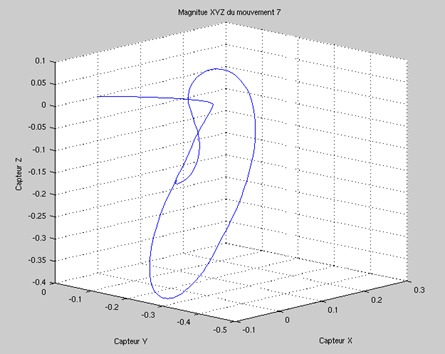
\includegraphics[width=10cm]{Ressources/Graphiques/MFB/Quaternions3D.png}
\end{center}
\vspace{0.5cm} 

Nous avons ensuite choisi les données les plus pertinentes en fonction de l'amplitude des signaux. Les signaux de la main ont été retenus puisque c'est avec ce capteur que les plus grands mouvements sont accomplis. Après avoir visualisé les données, les quaternions ainsi que le yaw le pitch et le roll ont été sélectionnées pour entrainer les HMM.
\\
\\
Comme les HMM prennent en compte l'aspect temporel des signaux, nous pouvons utiliser les signaux choisis sans faire une extraction de features.
Nous avons pourtant aussi essayé d'extraire les melcepst des signaux choisis. Cela peut paraitre surprenant puisque ce procédé est normalement réservé à la voix. Cependant, des résultats cohérents ont été obtenus avec cette technique...


%----------------------------------------------------------------------------------------
%	SECTION 3
%----------------------------------------------------------------------------------------
\section{HMM Implementation}

La structure du programme Matlab a été réalisée selon le laboratoire 3 que nous avons fait. Elle consiste à utiliser en parallèle autant de HMM que de mouvements à reconnaitre. Chaque HMM est entrainée séparément avec un type de mouvement.
\\
\\
Lors de la reconnaissance, une fonction compare le niveau de probabilité que chaque HMM retourne. Le mouvement qui correspond à la machine qui à le plus haut niveau de probabilité est choisi.

\begin{center} 
\hspace{15cm}
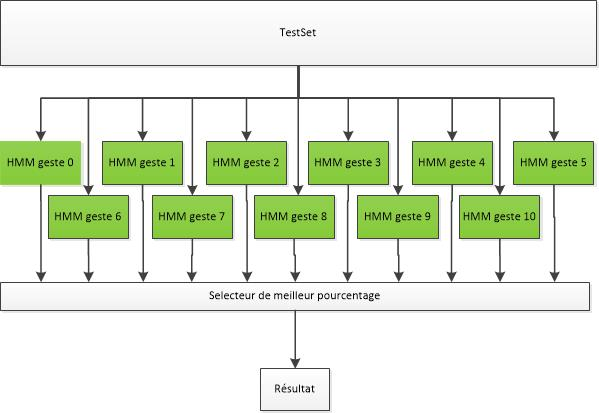
\includegraphics[width=15cm]{Ressources/Graphiques/MFB/HMMStructure.jpg}
\end{center}
\vspace{0.5cm} 

L'illustration ci-dessous décrit les différentes opérations effectuées lors de l'entrainement des HMM.

\begin{center} 
\hspace{15cm}
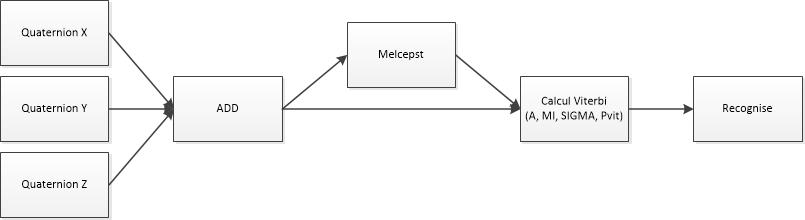
\includegraphics[width=15cm]{Ressources/Graphiques/MFB/TrainingStructure.jpg}
\end{center}
\vspace{0.5cm}


Dans un premier temps, nous additionnons les signaux. Puis nous calculons les melcepst. Nous entrainons ensuite la HMM avec l'algorithme de Viterbi et obtenons les matrices de transition, de moyenne, d'écart type ainsi que la probabilité de Viterbi. Finalement, nous effectuons la reconnaissance sur les gestes du set de données.
\\
\\
La première optimisation qui à été effectuée est l'augmentation du nombre d'itérations d'entrainement de la HMM avec l'algorithme de Viterbi. Après plusieurs essais, nous avons remarqué que les résultats convergeaient après 5 itérations. Il est donc inutile d'itérer plus que cinq fois pour avoir de bons résultats.
Après cette optimisation, le taux de reconnaissance est d'environ 30\%.
\\
\\
Le nombre d'état des HMM à été fixé à cinq pour toutes les machines. Nous avons essayé d'optimiser les réglages du nombre d'état pour arriver à un meilleur score en procédant par essai. Nous nous sommes basé sur la forme des signaux et les différentes phases de transition de ces derniers lors de l'exécution d'un mouvement.
\\
\\
Le taux de reconnaissance à progressé de 30\% à 50\% en ajoutant ou en enlevant des états à l'une ou l'autre des HMM . Cependant, aucune tendance n'est clairement apparue. Les changement étaient plutôt hasardeux, et cela même après l'analyse de la reconnaissance avec un histogramme. Cela peut s'expliquer par le choix des melcepst comme features, choix qui n'est peut-être pas adapté pour la reconnaissance des gestes avec les HMM.
\\
\\
On peut voir, sur le schéma que nous avons aussi essayé d'entrainer les HMM avec les données brutes.
Des essais ont également été effectués avec les données de yaw, pitch and roll.
Ces derniers essais n'ont rien donné de concluants, les résultats étaient pires qu'avant...


%----------------------------------------------------------------------------------------
%	SECTION 4
%----------------------------------------------------------------------------------------
\section{Performance and results}

Matlab n'a pas été facile à aborder. Son apprentissage s'est révélé difficile et cela a grandement freiné notre progression. La structure du programme était mauvaise. Il était difficile d'adapter notre programme pour pouvoir le télécharger et le lancer sur la plateforme Opegra. De plus, après avoir travaillé plusieurs jour sur ce projet, le temps venait à manquer, nous avons du stopper nos recherches. Pour toutes ces raisons, aucun score n'a été obtenu sur la plateforme Opegra.
\\
\\
Le meilleur score que nous avons obtenu sur notre ordinateur local est de 50\% de reconnaissance avec l'utilisation des melcepst comme features. Nous n'avons pas pu obtenir mieux. On peut expliquer cela par un mauvais choix des features. En effet, les melcepst sont souvent utilisés pour la voix, la progression des scores de reconnaissance a plafonné à 50\% peut-être parce-que ces features donne des résultats trop peu distincts.
\\
\\
Étonnement, les essais effectués avec les données brutes n'ont pas donné de résultats probants. Nous pensons que c'est la méthode avec laquelle les meilleurs résultats auraient du être obtenus. On peut expliquer l'échec de l'utilisation des données brutes par une faute d'implémentation dans l'algorithme de reconnaissance.


%----------------------------------------------------------------------------------------
%	SECTION 4
%----------------------------------------------------------------------------------------
\section{Possible improvement}

Beaucoup de choses peuvent être améliorées pour notre algorithme HMM.
\\
\\
Il faudrait commencer par s'assurer que l'algorithme fonctionne bien avec toutes les données (avec des données brutes ou des melcepst).
Pour cela Il faudrait restructurer le programme afin d'avoir une vision clair sur comment fonctionne le code.
\\
\\
A partir de là, nous pourrions recommencer à évaluer la pertinence des features choisies, puis le nombre d'états optimal pour chaque mouvement distinct.







